% !TEX root = document.tex

\chapter{\label{chap:introduction}Introduction}

Continuation-passing style is a time-tested paradigm of functional compilation \autocite{steele1978rabbit, DBLP:books/daglib/0022396}. It bridges the gap between high-level programming languages and (abstract) machine code. Primarily used for compiling first-class functions, CPS is flexible enough to compile many other language features. CPS is a style of programming, but can also be seen as a language in itself, namely a restricted form of the lambda calculus \autocite{barendregt1984lambda}. This fact gives it a solid theoretical foundation.

\begin{figure}
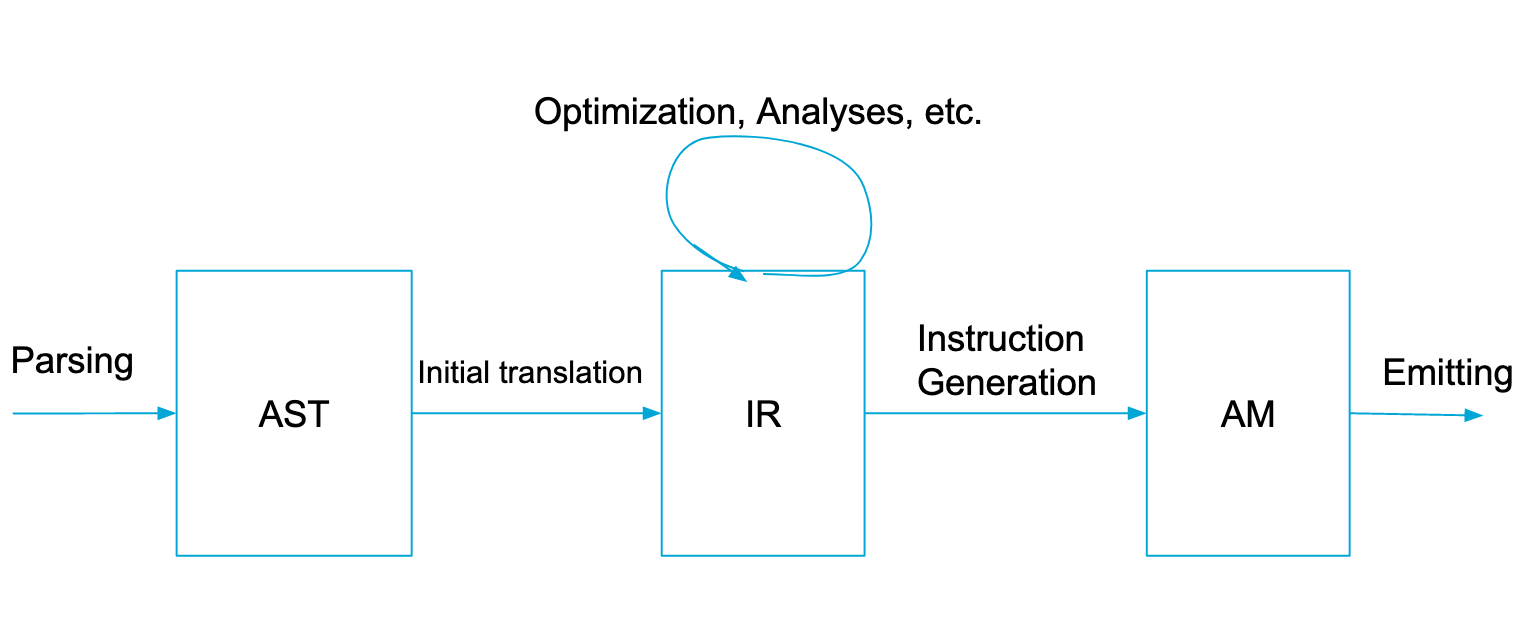
\includegraphics[width=1\textwidth]{./img/compiler_organisation.png}
\caption{Abstract compiler organization made up of Abstract Syntax Tree (AST), Intermediate Representation (IR), and Abstract Machine (AM)}
\label{fig:comporg}
\end{figure}

The language that is used by a compiler to represent source code is called an intermediate representation, as can be seen in figure \ref{fig:comporg}. A compiler writer uses an IR to implement optimizations and translations. An IR is designed to make compilation possible and pleasant. This is what CPS provides with its records and continuations. Resulting in a convenient abstraction for data flow and control flow \autocite{bruin2020framevm}. 

We will examine two improvements on CPS in this thesis: easier to write CPS conversion, and the ability to type transformations more strongly. The data structure we will use for this examination is a command tree \autocite{commandtreespoulsen}. Our command tree based IR will have a declarative front-end and a modular structure.

To validate the usefulness of the changes to our IR we will build a small compiler in Haskell \autocite{haskellhomepage} for WebAssembly \autocite{webassemblyhomepage}. Haskell implements languages using data structures, which formalize the specification of a language. Our source language will be the lambda calculus. Even though the lambda calculus is a very simple functional programming language, it has sufficient abstraction to necessitate compilation to a low-level langauge like WebAssembly. The first-class functions of the lambda calculus will need to be translated to the second-class functions of WebAssembly. The compiler will have multiple smaller translation steps and multiple passes over the IR. The translation from the lambda calculus to our IR and the elimination of first-class functions will demonstrate the usefulness of our IR.

The contributions of this thesis are the following:
\begin{itemize}
\item Two version of LamToWat: a WebAssembly compiler for the lambda calculus.
\item Command Trees as an IR for functional language compilation.
\end{itemize}

This thesis will continue with a chapter on the first version of the compiler based on CPS. In the third chapter we will go into some detail about command trees and show the improved version of the compiler. We will evaluate the improvements by comparing both versions of the compiler. In chapter \ref{chap:compiler} we will discuss validation and extension of our compiler. In chapter \ref{chap:related-work} we will discuss related work to support our analysis and give context to our compilation scheme.